\documentclass[a4paper,10pt]{jsarticle}

% 余白の設定
\setlength{\textwidth}{\fullwidth}
\setlength{\textheight}{40\baselineskip}
\addtolength{\textheight}{\topskip}
\setlength{\voffset}{-0.2in}
\setlength{\topmargin}{0pt}
\setlength{\headheight}{0pt}
\setlength{\headsep}{0pt}

% パッケージ
\usepackage[dvipdfmx]{graphicx}		% 画像
\usepackage{amsmath, amssymb}		% ギリシャ文字
\usepackage{bm}				% 数式
\usepackage{comment}			% コメント
\usepackage{siunitx}			% SI単位
\usepackage{framed}			% 枠組み
\usepackage{wrapfig}   %図の回り込み

% 表紙の設定
\makeatletter
\def\lst@lettertrue{\let\lst@ifletter\iffalse}
\def\@thesis{人工知能特論最終レポート}
\def\id#1{\def\@id{#1}}
\def\id#1{\def\@id{#1}}
\def\idone#1{\def\@idone{#1}}
\def\idtwo#1{\def\@idtwo{#1}}
\def\idthree#1{\def\@idthree{#1}}
\def\memberone#1{\def\@memberone{#1}}
\def\membertwo#1{\def\@membertwo{#1}}
\def\memberthree#1{\def\@memberthree{#1}}
\def\department#1{\def\@department{#1}}

\begin{document}
\def\@maketitle{
\begin{center}
  {\huge \vspace{100mm} \@thesis \par}
\end{center}
\begin{flushright}
  \vspace{170mm}
  {\Large \@date\par}                % 作成日
  {\Large \@department \par}         % 所属
\end{flushright}
\begin{flushleft}
  \hspace{113mm}
  {\large \@id}
  {\large \@author \par}               % 氏名
  \hspace{127mm}
  {\small \@idone}
  {\small \@memberone \par}            % 氏名
  \hspace{127mm}
  {\small \@idtwo}
  {\small \@membertwo \par}                  % 氏名
  \hspace{116mm}
  \hspace{1em}
  {\small \@idthree}
  {\small \@memberthree \par}                  % 氏名
  \vskip 1.5em
\end{flushleft}
}

% 表紙の中身
\makeatother
\date{\today}
\department{チーム : F}
\id{○ M18J4043M}
\author{中島 太知}
\idone{M18J4024Z}
\memberone{阪本 光翼}
\idtwo{M18J4026M}
\membertwo{佐藤 洸亮}
\idthree{M18J4059B}
\memberthree{三宅 裕稀}

\maketitle
\thispagestyle{empty}     %ページ番号削除
\clearpage
\addtocounter{page}{-1}

\newpage

\section{ゲームの説明}
\subsection{概要}
これは,順番に指定範囲内の数字を取り合っていき,
終了点に指定された数字を踏んだら負けとなる数取りゲームを木探索を用いたAIを相手に行うものである.
今回は探索を複雑にするため3人対戦で行い,人間の数とCOMの数は任意に決められるものとしている.
\subsection{ルール}
\begin{itemize}
  \item AIを含め3人対戦で行う.
  \item 終了点は任意で決められる.
  \item AIの強さは3段階で決められる.
  \item プレイ順はランダムで決まる.
  \item 1度に取れる数値は1か2のみ.
  \item 最終的に終了点の数を踏んだら負け.
\end{itemize}
以上のルールでゲームを行う.

\section{ゲームの定義}
\subsection{状態表現}
今回はコンソール上でゲームを行う.
よって状態表現はコンソール上に文字として表現する.
表示する状態はプレイヤーあるいはAIの選択した数値およびそれによって移動した後の現在地である.
また,1ターン終了度に誰がどの数値をとったかのログを表示する.

\subsection{オペレータ}
AIは強さに応じた先読みを行い,
より勝率が高い結果を返す.
返す結果は1か2である.
先読みした勝率が同等の場合,
もしくは先読みで結果が読みきれない場合はランダムで1か2を返すようにする.

\subsection{評価関数}
前述のように,AIの強さに応じて先読みを行うことで状況判断をおこなう.
今回プレイヤーの数を3人に設定したため,
AIが勝利するにはゲーム終了値から2つ手前の数を取ることができれば他プレイヤーが最小値を取得しても勝利することが可能である.
ゲーム終了値を11とした場合のAIの探索例を図\ref{fig:search}に示す.
プレイ順がプレイヤー1,プレイヤー2,AIの順であるとすると.
プレイヤー2が5を取得した場合,AIの選択できる数値は図のオレンジ色で示した数値である.
終了値が11であるためAIは9を取得すれば良いことになる.
よって図の最右端にあるAIの列が9になれば良い.
このように勝ち数が多くなる選択をすることでゲームを進行して行く.
\begin{figure}
  \centering
  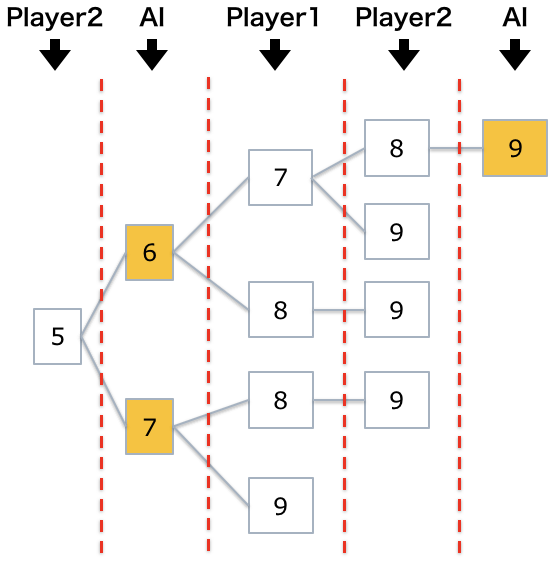
\includegraphics[width=100mm]{./image/AI_Search.png}
  \caption{探索の方法}
  \label{fig:search}
\end{figure}
\par
評価関数のプログラムには再起を用いた探索を利用し,AIの強さによって探索の深さを変更する.
プログラムの流れを図\ref{fig:Flow}に示す.
\begin{figure}
  \centering
  
\includegraphics[width=140mm]{./image/Search_Flow.png}
  \caption{評価関数の流れ図}
  \label{fig:Flow}
\end{figure}

\section{プログラムの概要}
\begin{wrapfigure}{r}{75mm}
  \centering
  
\includegraphics[width=50mm]{./image/Over_Flow.png}
  \caption{ゲームの全体の流れ図}
  \label{fig:over}
\end{wrapfigure}
今回,プログラムはC++を用いて設計した.
C++を用いた理由は,使い慣れていることと処理速度が早いことの2点である.\par
プログラムの全体の進行は図\ref{fig:over}に示すような流れとなる.\par
はじめにプレイヤー及びAIの情報入力を行う.
プレイヤー及びAIの情報管理は構造体を用いて行っている.
当初,配列を用いた管理を行おうと考えていたが,
プレイヤーが持つ情報が多く複雑になってしまうため,
構造体による管理に仕様を変更した. \par
プレイヤー情報及びAIの情報入力の次にゲームの設定を行う,
ここではゲームの終了点お設定とAIの強さを設定する.
最後にプレイ順をランダムで決定し,ゲームを開始する.
ゲームの中身は先ほど決定したプレイ順に現在の状態(数値)に1と2のどちらを加算するかを決定する動きをループで回すようにする.
また,1ターン終了度にログを表示していき,誰が何番の数字を取得したがわかるようにする. \par
加算されて行った数値が初めに設定した終了点に到達次第ゲームを終了し,
終了点の数値を取得してしまったプレイヤーを敗者とし,
最終的なゲームログを表示して終了とする.

\section{プログラムの設計}
\subsection{プレイヤー情報の格納}
初めに前述したプレイヤー及びAIの情報管理に用いた構造体について解説する.
構造体\textbf{\textit{MEMBER}}は\textit{Name}, \textit{Type}, \textit{Strength}の3つの要素で構成される.
要素Nameはchar型の変数でプレイヤー及びAIの名前を格納する.
要素Typeはint型の変数である.
要素Typeには"0"か"1"のどちらかの数値が格納され,"0"ならば人間,"1"ならばAIであると言う判定に用いる.
要素Strengthもint型の変数であり,要素Typeが"1",つまりAI用の構造体の時のみ使用される.
これはAIの強さの判定に用いられ,先読みが可能なターン数が格納される.
AIの強さが最弱の場合,一手先が読めるよう"2"が格納される.
これは後述する評価関数の仕様により[先読みするターン数 $\times$ 2]の数が格納される.
\subsection{プレイ順の決定}
このゲームはプレーヤーとAIを合わせて3プレーヤーで行う.
この時,プレイ順はランダム関数を用いて決定する.
プレイ順は全部で6通りであるため,ランダム関数によって0から5の数値を決定する.
プレイ順の変更にはポインタを用いる.
初めは構造体のポインタはプレイヤー情報を入力した順になっているため,
ランダム関数によって決定されたプレイ順に前述の構造体のポインタを入れ替えることでメインループにおける実行順を変更する.
図\ref{fig:Ch.Kouzoutai}は構造体の構成とその入れ替えの様子を示したものである.
\begin{figure}[h]
  \centering
  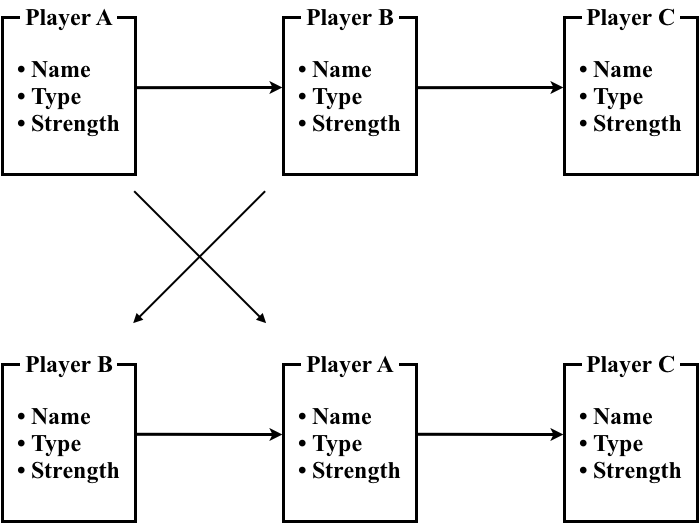
\includegraphics[width=120mm]{./image/Kouzoutai_Change.png}
  \caption{構造体の構成と入れ替え}
  \label{fig:Ch.Kouzoutai}
\end{figure}

\subsection{メインループ}
ゲーム進行を行うメインループの設計について解説する.
メインループ内は主に\textit{GetPlayer},\textit{GetAI},\textit{GetOperate},\textit{GetMemory}の4つの関数で構成されている.
\subsubsection{GetPlayer関数とGetAI関数}
GetPlayer関数とGetAI関数は主にプレイヤーへの指示及び状態の表示を行う関数であり,
bool型の関数である.
メインループも冒頭で呼び出され,
指定のポインターが示す構造体の要素Strengthが"0"か"1"を条件分岐により判定し,
関数GetPlayerか関数GetAIのいづれかに振り分ける.\par
関数GetPlayerでは現在の位置を表示後,
プレイヤーに+1か+2のどちらかを選択してもらう.
指定された数を現状態に加え,$True$を返す.
この時,変更後の現状態がゲーム終了点に達していれば$False$を返し,ゲームを終了させる.\par
一方,GetAI関数は構造体の要素$Strength$が"1"であり,AIのターンの場合に呼び出される.
GetAI関数内ではGetOperate関数を"1"を加える場合と"2"を加える場合で2回呼び出しており,
GetOperate関数によって得られた数値を比較し,
評価の高い結果を現状態に加える.
ただし,GetOperate関数によって得られた2つの数値が同じであった場合はランダムで加える数値を決定する.
この時,GetPlayer関数と同様に通常時$True$を返すが,
更新した現状態がゲーム終了値であれば$False$を返す.
\subsubsection{GetOperate関数}
GetOperate関数はGetAi関数内で呼び出されるvoid型の関数であり,
AIの評価関数に相当する.
この関数は再帰によって先の手を探索して行く.
探索の深さは構造体の要素$Strength$によって決定し,
1手先読み,4手先読み,全探索の3パターンが存在する.
ここでは4手先読みを例にアルゴリズムの説明をする.
図\ref{fig:AI_think}はAIが+1を選択し次のターンを探索する様子を表す図である.\par
思考するAIから見ると,
次のAIのターンに回ってくる可能性がある数は
$$[思考中のAIが選択した数字+思考中のAIを除いた2プレイヤーが選択した数値の合計]$$
である.
すなわち,
探索はAIが加算する範囲(1$\sim$2)と他のプレイヤーが選択する範囲(2$\sim$4)を交互に探索する形となる.
探索はAIが1を選んだ場合と2を選んだ場合の2パターンで行う.
それぞれの探索結果を比較しより良い結果が出る値を採択する.
4手先読みを行う時,
探索の深さを決定する変数\textbf{dep}には8が格納されている.
AIの選ぶ数別に探索を行うため初めの探索は他プレイヤーの選択する数値になる.
この時,
変数$dep=8$であり1階層分の探索を終える度にディクリメントを行う.
次は1手先のAIターンを探索する,
この時変数$dep$はディクリメントされ$dep=7$となる.
すなわち変数$dep$が偶数の時は他プレイヤーの探索,
奇数の時はAIの探索を行っている状態となる.
これを利用し,
$dep$が奇数の時に勝ち数を踏めた数の合計をグローバル変数$CNT$に格納する.
これを現在のターンで+1を選んだ場合と+2を選んだ場合とで比較することでより勝率の高い選択を行えるようになる.
この時,
両パターンの勝ち数が同数だった場合はランダムで選択する数値を決定することで単調なゲーム進行になることを防いでいる.
\begin{figure}[h]
  \centering
  
\includegraphics[width=140mm]{./image/AI_Think.png}
  \caption{GetOperate関数のアルゴリズム}
  \label{fig:AI_think}
\end{figure}
\subsection{GetMemory関数}
GetMemory関数はゲームログの表示を担う関数である.
実際のゲームログは,二次元配列$memory$に格納される.
配列$memory$は$3\times32$の二次元配列であり,
プレイヤーごとの取得した数値を保管して行く.
ログはプレイ順に格納されて行くためGetMemory関数では配列の中身を順に表示するだけで良い.
図\ref{fig:memory}は配列memoryに格納されたログの例を示している.
GetMemory関数は毎ターン終了時およびゲーム終了時に呼び出される.
\begin{figure}
  \centering
  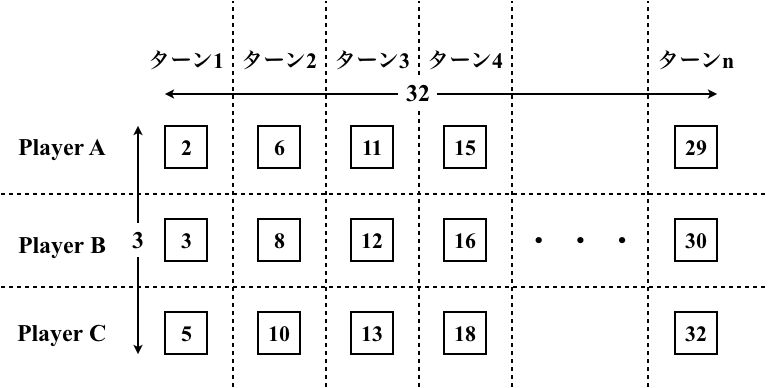
\includegraphics[width=120mm]{./image/memory.png}
  \caption{配列memoryの中身}
  \label{fig:memory}
\end{figure}

\section{実装結果}
実際にシステムを実装した結果を示す.
今回は人間1:COM2とCOMのみでゲームを行なった.
\subsection{動作テスト}
図\ref{fig:GameSet}はゲームの初期設定を行なっている場面である.
ユーザー情報入力時では構造体にPlayer\_A,COM\_A,COM\_Bの順に情報が格納されているが,
順番の変更に伴ってCOM\_A,COM\_B,Player\_Aの順に変更されていることがわかる.
今回ゲーム終了点は24,AIの強さはCOM\_Aを弱い,COM\_Bを強いに設定した.
図\ref{fig:GameResult}は全体のゲーム進行の様子および最終的な結果である.
結果はCOM\_Aの敗北となり,AIの強さに従った結果となった.
毎ターン表示されるゲームログもプレイ順に正しく表示されている.
ゲーム終了時のログ図\ref{fig:GameResult}の最下部にあるように未プレイのプレイヤーのログには何も表示されないようになっている.
また,図\ref{fig:GameMiss}はゲーム中のエラー処理の様子であり,
プレイヤーが範囲外の数値を指定してしまった場合に,
正しい数値を指定するように促すようになっている.\par
次にAIのみで対戦を行い,
強さを変更しながら結果を観察した.
終了点は全て24で行っている.
設定ごとの結果を以下に示す.
\begin{description}
  \item[弱いvs弱いvs強い]\mbox{}\\
  この設定では強いAIが弱いAIに敗北することはなかった.
  弱いAIのどちらが負けるかはランダムであった.
  \item[弱いvs普通vs強い]\mbox{}\\
  勝敗はAIの強さとは関係なくランダムであった.
  \item[普通vs普通vs強い]\mbox{}\\
  基本的に普通のAIのどちらかが敗北した,
  しかし数回に1回の頻度で強いAIも敗北していた.
  強いAIが敗北する頻度は[弱いvs普通vs強い]の時よりも低く感じた.
  \item[弱いvs弱いvs弱い]\mbox{}\\
  勝敗は完全にランダムであった.
  \item[普通vs普通vs普通]\mbox{}\\
  上述の[弱いvs弱いvs弱い]と同様に勝敗は完全にランダムであった.
  \item[強いvs強いvs強い]\mbox{}\\
  必ずプレイ順が2番手となったCOMが敗北した.
\end{description}
以上が今回の実装で得られた結果である.
\begin{figure}[htbp]
  \begin{minipage}{0.5\hsize}
    \centering
    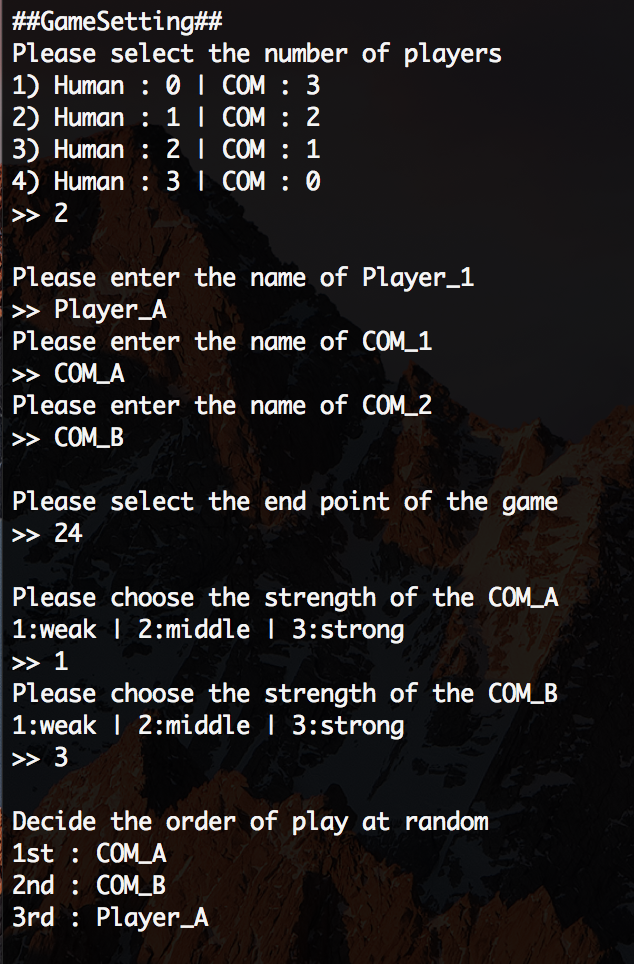
\includegraphics[width=70mm]{./image/GameSet.png}
    \caption{ゲームの初期設定部分の例}
    \label{fig:GameSet}
    \vspace{7em}
    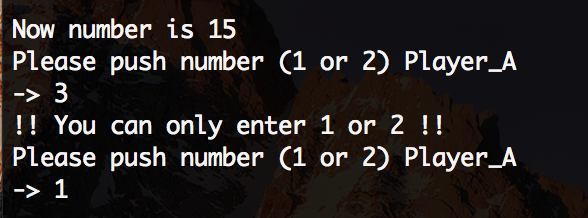
\includegraphics[width=70mm]{./image/GameMiss.png}
    \caption{エラー処理}
    \label{fig:GameMiss}
  \end{minipage}
  \begin{minipage}{0.5\hsize}
    \centering
    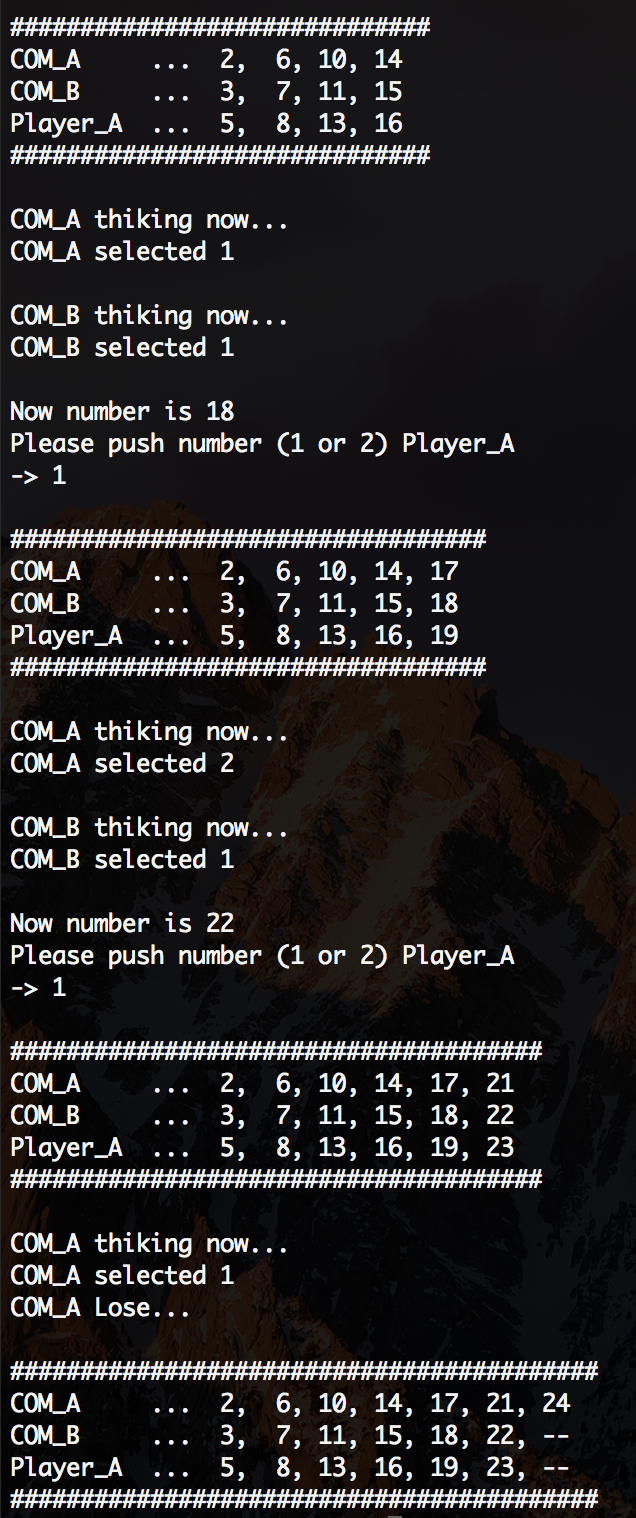
\includegraphics[width=70mm]{./image/GameResult.png}
    \caption{ゲームの流れと結果}
    \label{fig:GameResult}
  \end{minipage}
\end{figure}
\subsection{考察}
今回得られた結果から,1手先しか読むことのできないAIは実際に最弱ではあるが,
4手先読みが可能なAIと全探索が可能なAIでは大きく強さに差が出ないことがわかった.
これはゲームの特性上,前半の数値の選択による勝敗への影響が少ないため,
ある程度の探索ができれば強さへの影響も小さくなってしまうのではないかと考えた.\par
また,全て同じ強さに統一した時に\textbf{強い}の時のみ結果が変わらなかったのは,
全てのAIが全探索を行ってしまうため,
ゲーム毎の数値選択に変化が現れずプレイ順によって結果が固定しまったと思われる.\par
探索に関しては,+1を選んだ方が分岐の回数も置くなり,
必然的に+2を選ぶより多くの勝ち数を踏む可能性が高くなる.
そのため,最終局面以外でのAIの選択は+1が多くなる.
ゲームに抑揚を持たせるためにも,
+1と+2のパターンで探索に重み付けを行えばゲームの進行に抑揚が生まれるように思われた.

\section{結論}
このゲームには必勝法に近いゲーム展開が存在するため,考えてゲームを進行すれば人間がAIに負けることはなさそうであった.
今回はゲーム終了点を24に設定したが,
終了点が100などの大きな数字になると全探索を行うのにかなりの時間を要してしまった.
前述したようにゲームの特性上,
選択がゲームに及ぼすのは後半のみであるため,
このゲームには全探索を行うメリットはあまりなかったと考えられる.
そのためAIの探索深度は1手先読み,3手先読み,5手先読み程度の小さい範囲でのバランスが良さそうである.


\end{document}
